\chapter{Asymptotic notation}

In order to characterize the complexity of algorithms, it is useful to use
asymptotic big-O notation. Consider two functions $f, g \colon \NN \to \RR$. We
say that $f$ is $O(g)$ if and only if there exists a constant $C > 0$ and a
natural number $n_{C}$ such that the inequality $0 \le f(n) \le C\cdot g(n)$
holds for all $n > n_{C}$ \cite{clrs}.

It is common to write $f=O(g)$ instead
of ``$f$ is $O(g)$'', slightly abusing the mathematical notation \cite{clrs}.
One should notice that big-O notation does not provide a tight bound. For
instance, we have $n + 1 = O(n)$ (since $n + 1 \le 2 \cdot n$) but also $n+1 =
  O(n^{10})$.

In the context of computational complexity, big-O notation is most commonly
used for expressing upper bound on number of (dominating) operations performed
by an algorithm as a function of its input size $N$. Since the number of
performed operations is roughly proportional to the algorithm's execution time,
it follows that algorithms with better bound can be considered as more
performant. However, care must be taken when applying this reasoning to judge
practical performance. In particular, one should be mindful of the constant
factor $C$ in the definition above, as well as any bottlenecks stemming from
the working of the underlying hardware. As a concrete example, Strassen's
algorithm for multiplying two $N \times N$ matrices requires $O(N^{\alpha})$
multiplications, where $2 < \alpha < 3$, and yet may perform worse than naive
algorithm peforming $N^{3}$ multiplications, even for $N$ of order of several
hundreds \cite{dalberto}.

We conclude this section by mentioning that there exist several other
asymptotic notations. For instance, $\Omega$, describing the asymptotic lower bound
of a function, and $\Theta$ combining big-O and $\Theta$. For more details, we
refer the reader to \cite{clrs}.

\chapter{Conditional probability on square lattice}
\chaptermark{Conditional probability}
\label{sec:probability}
\begin{figure}
  \centering
  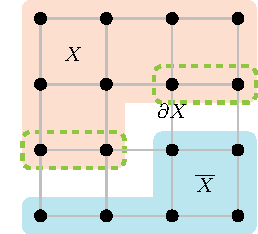
\includegraphics[width=0.6\textwidth]{figures/latticeonly}
  \caption{An example Ising spin-glass of 16 spins on a square lattice. The conditional
    probability for spins in the region $\overline{X}$ conditioned on the values of spins in the
    region $X$ depends only on the configuration on the border $\partial X$.}
  \label{fig:lattice}
\end{figure}

Consider a square lattice, such as the one depicted in Fig. \ref{fig:lattice}.
We will prove that the conditional probability for spins in the region $\overline{X}$
conditioned on the values of spins in the region $X$ depends only on the configurations of the spins on the
border $\partial X$.

Let denote by $H_X$ the usual Hamiltonian $H$ restricted to the graph
induced by vertices in $X$. Further, let $H_{X, \overline{X}} = H - H_X -
  H_{\overline{X}}$. Notice that $H_{X, \overline{X}}$ contains only quadratic
terms $J_{ij} s_i s_j$ such that $i \in X$ and $j \in \overline{X}$. Slightly
abusing the notation, one may thus write
\begin{equation}
  \small
  H(s_1, \ldots, s_N) = H_X(s_1, \ldots, s_k) + H_{\overline{X}}(s_{k+1}, \ldots, s_N) + H_{X, \overline{X}}(s_1, \ldots, s_N)
\end{equation}
Using definition of conditional probability applied to Boltzmann distribution,
one thus gets

\begin{align}
   & p(s_{k+1}|s_1, \ldots, s_k) = \frac{\sum\limits_{(z_{k+2}, \ldots, z_N)}e^{-\beta H(s_1, \ldots, s_{k+1}, z_{k+2},\ldots,z_N)}}{\sum\limits_{(z_{k+1}, \ldots, z_N)}e^{-\beta H(s_1, \ldots, s_k, z_{k+1},\ldots,z_N)}}                                                                                                                         \\
   & = \frac{\sum\limits_{(z_{k+2}, \ldots, z_N)}e^{-\beta (H_X(s_1, \ldots, s_k) + H_{\overline{X}}(s_{k+1}, z_{k+2},\ldots,z_N) + H_{X, \overline{X}}(s_1, \ldots, z_N))}}{\sum\limits_{(z_{k+1}, \ldots, z_N)}e^{-\beta (H_X(s_1, \ldots, s_k) + H_{\overline{X}}(z_{k+1}, \ldots,z_N) + H_{X, \overline{X}}(s_1, \ldots, z_N))}}                 \\
   & = \frac{e^{-\beta H_X(s_1, \ldots, s_k)}\sum\limits_{(z_{k+2}, \ldots, z_N)} e^{-\beta(H_{\overline{X}}(s_{k+1}, z_{k+2},\ldots,z_N) + H_{X, \overline{X}}(s_1, \ldots, z_N))}}{e^{-\beta H_X(s_1, \ldots, s_k)}\sum\limits_{(z_{k+1}, \ldots, z_N)}e^{ -\beta(H_{\overline{X}}(z_{k+1}, \ldots,z_N) + H_{X, \overline{X}}(s_1, \ldots, z_N))}} \\
   & = \frac{\sum\limits_{(z_{k+2}, \ldots, z_N)} e^{-\beta(H_{\overline{X}}(s_{k+1}, z_{k+2},\ldots,z_N) + H_{X, \overline{X}}(s_1, \ldots, z_N))}}{\sum\limits_{(z_{k+1}, \ldots, z_N)}e^{ -\beta(H_{\overline{X}}(z_{k+1}, \ldots,z_N) + H_{X, \overline{X}}(s_1, \ldots, z_N))}}
\end{align}
Note, in both numerator and denominator, spins with indices from $X$ appear
non-trivially only in $H_{X, \overline{X}}$ , i.e. the whole expression depends
only on those spins in $X$ that directly interact with spins in $\overline{X}$,
which was to be shown.

\chapter{Dispatching conditions}
\label{chapter:dispatching}
In the following appendix, we use the notation from chapter \ref{chapter:trains}.
\section{The minimum passing time condition.}
Any train $j$ cannot travel through a block $b \in \Bj$ faster than the corresponding minimum
passing time:
\begin{equation}
  \label{eq:dc1}
  \tout(j, b) \ge \tin(j, b) + \pmin(j, b).
\end{equation}
Using \eqref{eq:djs} and \eqref{eq:pt} one can easily verify that inequality
\eqref{eq:dc1} is equivalent to the following inequality for station blocks:
\begin{equation}
  \label{eq:passingtime}
  d(j, s_{j,k+1}) \ge d(j, s_{j,k}) - \sum_{b}\alpha(j, b),
\end{equation}
where the sum runs over all blocks starting form the one succeeding $s_{j,k}$
and ending in $s_{j,k+1}$.
In binary variables, it means that if, for a fixed $j,s,m$, the $x_{j,s,m}=1$,
then delays $d(j,s)$ smaller than $m-\sum_{b}\alpha(j, b)$ are prohibited
and thus the corresponding variables have to zero out. Hence, we arrive at the
following condition:
\begin{equation}
  \label{eq:qubo:passingtime}
  \forall_{j} \forall_{s \in S_j \setminus \{s_{{j,\eend}}\}}
  \sum_{m \in A_{j,s}}
  \left(
  \sum_{ m' \in D(m) \cap A_{j, s_{j,k+1}}} x_{j, s, m}
  x_{j, s_{j,k+1}, m'} \right) = 0,
\end{equation}
where $D(m) = \{0, 1, \ldots, m - \sum_{b}\alpha(j, b) -1\}$.
\section{The single block occupation condition.}
Two trains cannot occupy the same line block. Consider two
trains, $j, j' \in \JJ_0$ leaving the same station $s_{j,k} \in \Sj$ in the direction of the
next station block $s_{j,k+1}$. Suppose further that the train $j$ leaves
first. i.e. $\tout(j', s) > \tout(j, s)$. Since two trains cannot occupy the
same block, some headway time has to pass after $\tout(j, s)$ before the
train $j'$ can leave. This headway is dependent on both $j$ and a
sequence of blocks, and hence we denote it by $\tauu(j, s_{j,k})$. Thus,
the condition becomes:
\begin{equation}
  \label{eq:single-block}
  \tout(j', s_{j,k}) \ge \tout(j, s_{j,k}) + \tauu(j, s_{j,k}).
\end{equation}
Substituting for $\tout$ in \eqref{eq:single-block} yields the following
inequality for delays:
\begin{equation}
\begin{split}
  \label{eq:single-block-delays}
  d(j', s_{j,k}) &\ge d(j, s_{j,k}) + \ttout(j, s_{j,k}) - \ttout(j', s_{j,k}) + \\
  &+\tauu(j, s_{j,k})
\end{split}
\end{equation}
or,
\begin{equation}
  d(j', s_{j,k}) \ge d(j, s_{j,k}) + \Delta(j, j',s_{j,k}) + \tauu(j, s_{j,k})
\end{equation}
where
\begin{equation}
  \label{eq:delta}
  \Delta(j, j', s_{j,k}) = \ttout(j, s) - \ttout(j', s)
\end{equation}
The precise form of the headway $\tauu$ depends on the dispatching detail of the problem.
In our approach, we propose the following form:
\begin{equation}
  \tauu(j, s_{j,k}) = \max_{b}\{\pt(j,b)\}
\end{equation}
where the maximum is taken over all blocks between stations $s_{j,k}$ and $s_{j,k+1}$.
For our decision variables, we use a similar scheme as with the previous
constraint and the condition becomes:
\begin{equation}
  \label{eq:qubo:singleblock}
  \forall_{i=0,1} \forall_{j, j' \in \JJ^{i}} \forall_{s \in S^{*}_{j} \cap S^{*}_{j'}} \sum_{m \in A_{j, s}} \left(
  \sum_{m' \in B(m) \cap A_{j', s}} x_{j,s,m}x_{j',s,m'}
  \right) = 0,
\end{equation}
where, as previously, $\Sjs = \Sj \setminus \{s_{j,\eend}\}$, and $B(m) = \{m + \Delta(j, j', s), m + \Delta(j, j', s)+ 1,\ldots, m +
  \Delta(j, j', s) + \tau_{(1)}(j,s)-1 \}$
is a set of delays violating condition \eqref{eq:single-block-delays}.


\section{The deadlock condition}
The deadlock condition is analogous to the single block occupation condition
but for trains going in opposite directions. Suppose trains $j$ and $j'$ are
heading in opposite directions on a route determined by two consecutive
stations $s_{j,k}$ and $s_{j,k+1}$. Note that for $j'$ the order is reversed, i.e. it
starts at $s_{j,k+1}$ and travels in the direction of $s_{j,k}$. In this case, if $j$
is supposed to to leave $s_{j,k}$ before $j'$ leaves $s_{j,k+1}$, the following
condition has to be satisfied:
\begin{equation}
  \label{eq:deadlock}
  \tout(j', s_{j,k+1}) \ge \tout(j,s_{j,k}) + \tauuu(j, s),
\end{equation}
where $\tauuu(j, s_{j,k})$ is the minimum time required for train $j$ to
get from station block $s_{j,k}$ to $s_{j,k+1}$. Rewritten in terms of delays, the
inequality \eqref{eq:deadlock} reads:
\begin{equation}
  \label{eq:deadlock2}
  d(j',s_{j,k+1}) \ge d(j, s_{j,k}) + \Delta(j,j',s) + \tauuu(j, s).
\end{equation}
In decision variables, the deadlock condition in its basic form looks as
follows:
\begin{equation}
  \label{eq:qubo:deadlock}
  \forall_{s \in S^{*}_{j} \cap S^{*}_{j'}} \sum_{m \in A_{j, s}} \left(
  \sum_{m' \in C(m) \cap A_{j', s}} x_{j,s,m}x_{j',s,m'}
  \right) = 0,
\end{equation}
and has to be applied for a limited number of trains $j \in \JJ^{0} (\JJ^{1})$
and $j' \in \JJ^{1}(\JJ^{0})$. Here, $C(m)$ is, similarly to $B(m)$, the set of delays
violating the condition for the given pair.
\section{The rolling stock circulation condition}
Our model assumes that some trains might be assigned the same train set. Naturally,
there exists some necessary \emph{turnover time}, before a train set can be
reused. Formally, if trains $j$ and $j'$ going in opposite directions are
assigned the same train set, then the following inequality has to hold:
\begin{equation}
  \tout(j', s_{j',1}) > \tout(j, s_{j,\eend}) + \Delta(j, j')
\end{equation}
where $\Delta(j, j')$ is the minimum turnover time. In the delay
representation, the inequality becomes:
\begin{equation}
  \label{eq:rolling}
  \begin{split}
    d(j',s_{j',1}) + \ttout(j',s_{j',1}) > & \; d(j, s_{j,\eend-1}) + \ttout(j, s_{j,\eend-1}) + \\
    & \; \tauuu(j, s_{j,\eend-1}) + \Delta(j,j').
  \end{split}
\end{equation}
Inequality \eqref{eq:rolling} can be simplified to:
\begin{equation}
  d(j',s_{j',1}) > d(j, s_{j,\eend-1}) - R(j,j'),
\end{equation}
by setting:
\begin{equation}
  \label{eq:rolling2}
  \begin{split}
    R(j, j') \coloneq &\ttout(j',s_{j',1}) - \ttout(j, s_{j,\eend-1}) \\
    &- \tauuu(j,s_{j,\eend-1}) - \Delta(j,j').
  \end{split}
\end{equation}
In decision variables, the rolling stock circulation condition for trains $j$
and $j'$ can be written as
\begin{equation}
  \label{eq:qubo:rollingstock}
  \sum_{m \in A_{j, s_{(j, \eend-1)}}} \sum_{m' \in E(d) \cap A_{j',s_{(j',1)}}} x_{j,s_{(j,\eend-1)},m}x_{j', s_{(j',1)},m'} = 0
\end{equation}
where $E(d) = \{0, 1, \ldots, m-R(j, j')\}$.

\section{The capacity condition}
Let $s$ be a station block with $b$ tracks and let $\{j_{1},\ldots,j_{b+1}\} \subset \JJ$ be any $b+1$-tuple of
trains. There should not exist time $t$ for which all the following conditions are simultaneously satisfied:
\begin{equation}
  \begin{split}
    \tin(j_{1}, s) \le &t \le \tout(j_{1}, s) \\
    &\ldots \\
    \tin(j_{b+1}, s_{j,k}) \le &t \le \tout(j_{b+1}, s).
  \end{split}
\end{equation}
In delay representation, the conditions read:
\begin{equation}
  \label{eq:buffer}
  \begin{split}
    d(j_{1}, s_{j_{1},k_{1}-1}) &+ \ttout(j_{1},s_{j_{1},k_{1}-1}) \le t \\
                            &\le d(j_{1},s_{j_{1},k_{1}}) + \ttout(j_{1},s_{j_{1},k_{1}})\\
    \ldots \\
    d(j_{b+1}, s_{j_{b+1},k_{b+1}-1}) &+ \ttout(j_{b+1},s_{j_{b+1},k_{b+1}-1}) \le t \\
                            &\le d(j_{b+1},s_{j_{b+1},k_{b+1}}) + \ttout(j_{b+1},s_{j_{b+1},k_{b+1}}),
  \end{split}
\end{equation}
where $k_{j_{i}}$ is the index of station $s$ in sequence $\Sj$.

The condition \eqref{eq:buffer} translated into binary variables can give a lot of additional terms.
In our problem instances, we ignore this condition, but verify the obtained solutions against it.
%%% Local Variables:
%%% mode: latex
%%% TeX-master: "../main"
%%% End
